\documentclass{article}
\usepackage{amsmath,amssymb,amsfonts,amsthm}
\usepackage{graphicx,multirow}
\usepackage{framed}
\usepackage{color,xcolor}
\usepackage{mathtools,wrapfig,multicol,geometry}
%{
%\hyphenpenalty=1000
%\oddsidemargin -0.1in %-0.4in for smaller margins
%\topmargin -0.8in %-1in (for above)
%\textheight 10.75in %10.75in (for above)
%\textwidth 6.5in %6.75in (for above)
%\parindent=0pt

\pagestyle{headings}%{headings}if you want page numbers top right
\graphicspath{{pictures/}}
%%页边距
\geometry{left=2.0cm, right=2.0cm, top=2.0cm, bottom=2.0cm}
%***************************************************************************
\newcommand{\ds}{\displaystyle}%display maths
\newcommand{\sst}{\scriptstyle}%very small maths
\newcommand{\sm}{\textstyle}%normal size maths
\newcommand{\bm}[1]{\mbox{\boldmath{$#1$}}}
\newcommand{\rom}[1]{\mbox{${\rm#1}$}}%roman in maths
\newcommand{\sech}{\rom{sech}}
\newcommand{\cosech}{\rom{cosech}}
\newcommand{\cosec}{\rom{cosec}}
\newcommand{\pa}{\partial}
\newcommand{\ep}{\varepsilon}
\newcommand{\na}{\bm\nabla}
\newcommand{\ns}{\nabla^2}
\newcommand{\p}{\prime}
\newcommand{\pp}{\prime\prime}
\newcommand{\ppp}{\prime\prime\prime}
\newcommand{\cc}{C$^{_{\!\!\!\!\!\vert}}$ \ }
\newcommand{\hf}{$\!\!\!\!$\qquad \hfill}
\newcommand{\vf}{$\!\!\!\!$\quad\vfill}

% Define the \nth command.
\makeatletter
\newcount\T@stCount             \newcount\TestCount
\def\nth#1{%
     \def\reserved@a##1##2\@nil{\ifcat##1n%
            0%
    \let\reserved@b\ensuremath
       \else##1##2%
    \let\reserved@b\relax
       \fi}%
     \TestCount=\reserved@a#1\@nil\relax
     \ifnum\TestCount <0 \multiply\TestCount by\m@ne \fi % subdue negatives
     \T@stCount=\TestCount
     \divide\T@stCount by 100 \multiply\T@stCount by 100
     \advance\TestCount by-\T@stCount     % n mod 100
     \ifnum\TestCount >20 \T@stCount=\TestCount
       \divide\T@stCount by 10 \multiply\T@stCount by 10
       \advance\TestCount by-\T@stCount   % n mod 10
     \fi
      \reserved@b{#1}%
        \textsuperscript{\ifcase\TestCount th%    0th
                         \or   st%                1st
                         \or   nd%                2nd
                         \or   rd%                3rd
                         \else th%                nth
                         \fi}%
      }

\newenvironment{remark}[1][Remark]{\begin{trivlist}
\item[\hskip \labelsep {\bfseries #1}]}{\end{trivlist}}
%***************************************************************************
%***************************************************************************
\pagestyle{myheadings}%for header and pagenumber with \markright{\rm...{  }}
\markright{\textit{\sffamily{MTH 208 \hspace{1cm}  \textbf{Numerical Analysis}}}}
%use with \thispagestyle{empty} after begin document
%***************************************************************************
%***************************************************************************
\begin{document}
\thispagestyle{empty}%If 1st page requires no number
%***************************************************************************
\sffamily
\begin{flushleft}
%***************************************************************************  %@@
\begin{figure}
    \centering
		\includegraphics[width=0.50\textwidth]{XJTLU}
	\label{fig:XJTLU}
\end{figure}

%***************************************************************************  %@@
{\Large {\textbf{MTH208: Coursework II Solution Sheet (15 \%)} \hfill }}\\%dont to change these  %@@
\vspace*{0.2cm}  %@@
\hrule
\vskip0.02cm
\hrule  %@@
\vskip0.4cm  %@@
%***************************************************************************  %@@Name:$\underline{\hspace{2cm}}$ Student ID:$\underline{\hspace{2cm}}$
%***************************************************************************  %@@
{\textbf{\large {Year:$\;$ 2023  \quad Name:$\;$ $\underline{Zhenpeng.Liu20}$\quad ID:$\;$ $\underline{2033519}$  }}\\
\center{\bf
Instructions on the Coursework}} \\[0.7cm]
\begin{itemize}
  \item Total marks for the coursework  are 15. There are 2 comprehensive questions in the exam. Please write down detailed solution process and submit your completed solution via a submission link provided on the LMO. You may complete the work by using the provided solution sheet in word or tex.
  \item  All the learning materials on the LMO can be
referenced during the exam including lecture notes, Lab codes,
lecture videos etc. However, you must complete the coursework independently.
 \item Please name your submission in the form {\text MTH017Final+ID+ZhangSan.pdf}
\item The coursework will be available on 9:00AM May 10th and deadline for submission is 9:00AM  May 19th.
\end{itemize}

\begin{enumerate}
\item Question I: Numerical Quadrature.
\begin{framed}
\textcolor{blue}{ Solution: }
We call the following integrals:
\[
  f_{c}(x) = \frac{\cos(x)}{\sqrt{x}} ,and \quad f_{s}(x) = \frac{\sin(x)}{\sqrt{x}}
\]
\[
  I_{c} \coloneqq \int_{0}^{1} \frac{\cos(x)}{\sqrt{x}} \,dx = \int_{0}^{1} f_{c}(x) \,dx, and\quad
  I_{d} \coloneqq \int_{0}^{1} \frac{\sin(x)}{\sqrt{x}} \,dx = \int_{0}^{1} f_{s}(x) \,dx,
\]
%-------------------------------Q(1-a)
\rule[-0.7mm]{45em}{0.5pt}
(1-a)
\newline
Firstly, let's `ignoring' the singularity at \(x=0\), which means let \(f(0) = g(0) = 0\) in the trapezonidal rule method calculation. And use this function with n intervals of equal length \(h = 1/n\)

\begin{multicols}{2}
\begin{verbatim}
function I = trapez_1a(f,n)
% assume f is vectorized
h = 1/n;
x = linspace(0,1,n+1);
%let f(0)=0
I = 0 + f(1);
I = I + 2*sum(f(x(2:end-1)));
I = I*h/2;
end
\end{verbatim}
\columnbreak
\begin{verbatim}
n = 100:10:1000;
fc = @(x) cos(x)./sqrt(x);
fs = @(x) sin(x)./sqrt(x);
Ic_a = zeros(1,length(n));
Is_a = zeros(1,length(n));
index = 1;
for i = n
    Ic_a(index) = trapez_1a(fc,i);
    Is_a(index) = trapez_1a(fs,i);
    index = index+1;
end
\end{verbatim}
\end{multicols}


%翻页

%第二页
\newpage
Then we plot \(I_{c}\) \(I_{s}\) depend on \(n\) (\(n\) can be hundards to 1000)
\newline
\begin{multicols}{2}
\begin{verbatim}
n = 100:10:1000;
fc = @(x) cos(x)./sqrt(x);
fs = @(x) sin(x)./sqrt(x);
Ic_a = zeros(1,length(n));
Is_a = zeros(1,length(n));
index = 1;
for i = n
    Ic_a(index) = trapez_1a(fc,i);
    Is_a(index) = trapez_1a(fs,i);
    index = index+1;
end
save("1_a","Is_a","Ic_a");
\end{verbatim}
\columnbreak
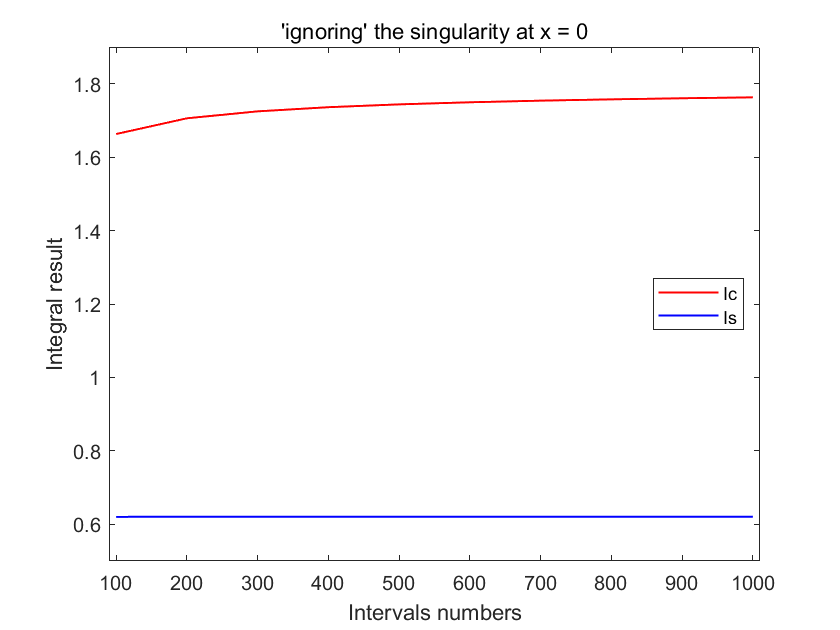
\includegraphics[width={0.9\linewidth}]{Q1_a.png}
\end{multicols}
\verb|fprintf('For n = 1000:\nIc_a is %.4f\nIs_a is %.4f\n',Ic_a(end),Is_a(end))|
\newline
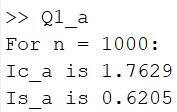
\includegraphics[width={0.15\linewidth}]{Q1_a_sol.png}
\newline
We can observe that the error on [0,h] is \(\int_{0}^{1} f(x) \,dx - \frac{1}{2}h \cdot f(h)\). It will decrease by increasing n.
\newline
And the error on [h,1] will decrease by increasing n too.
\newline
For \(Ic\), the initial error is large because \(\lim_{x \to 0}f_{c}(x) = \inf\), but we consider its singularity as 0. So the error on [0,h] will be big.
For \(Is\), the initial error is small because \(\lim_{x \to 0}f_{s}(x) = 0\), so we consider its singularity as 0 is reasonable.
\newline
So it is a good way to approximate calculate Is, but not work good for \(Ic\).
\rule[-0.7mm]{45em}{0.5pt}
%-------------------------------Q1_b
\newline
(1-b)
\newline
Secondly, we will treat the function on [0,h] as \(w(x) = x^{-1/2}\), and preserve the function on [h,1]. Notice that we can calculate directly that \(\int_{0}^{h}=2\sqrt{h}\).

\begin{multicols}{2}
\begin{verbatim}
function I = trapez_2a(f,n)
% assume f is vectorized
h = 1/n;
% on [h,1]
x = linspace(0,1,n+1);
x = x(2:end);
I1 = f(x(1)) + f(x(end));
I1 = I1 + 2*sum(f(x(2:end-1)));
I1 = I1*h/2;
% on [0,h]
I0 = 2.*sqrt(h);
I = I0+I1;
end
\end{verbatim}
\columnbreak
\begin{verbatim}
n = 100:10:1000;
fc = @(x) cos(x)./sqrt(x);
fs = @(x) sin(x)./sqrt(x);
Ic_b = zeros(1,length(n));
Is_b = zeros(1,length(n));
index = 1;
for i = n
    Ic_b(index) = trapez_2a(fc,i);
    Is_b(index) = trapez_2a(fs,i);
    index = index+1;
end
save("1_b","Is_b","Ic_b");
\end{verbatim}
\end{multicols}
Then we plot \(I_{c}\) \(I_{s}\) depend on \(n\) (\(n\) can be hundards to 1000), And compare with the data from (1-a)
\begin{verbatim}
plot(n,Ic_b,'Color',"#A2142F","LineWidth",1);
hold on
plot(n,Is_b,'Color',"#0072BD","LineWidth",1)
hold on
load 1_a.mat
plot(n,Ic_a,'--r',n,Is_a,'--b',"LineWidth",0.6);
axis([90 1010 0.5 1.9]);
title('Treat [0,h] as w(x)');
xlabel('Intervals numbers');
ylabel('Integral result');
legend('Ic_b','Is_b','Ic_a','Is_a','Location','East')
\end{verbatim}
\begin{multicols}{2}
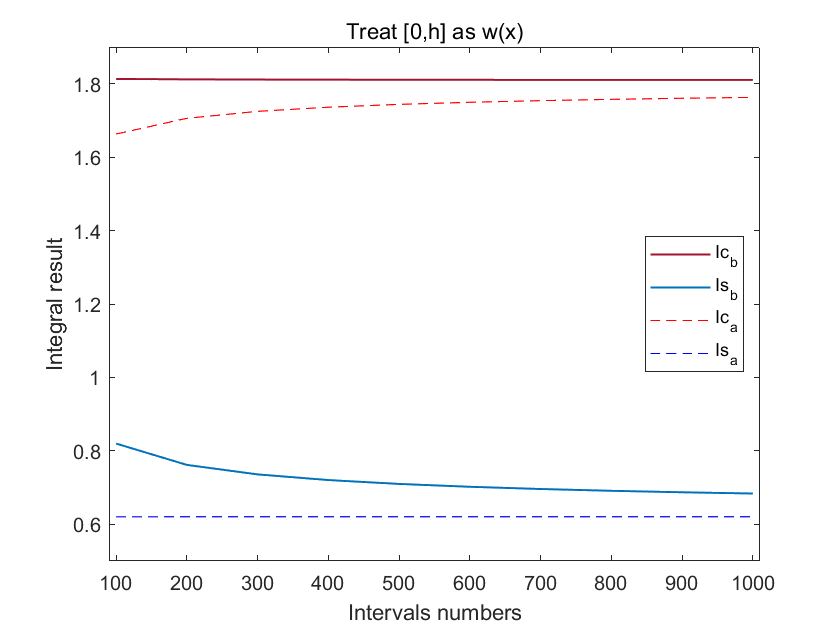
\includegraphics[width={\linewidth}]{Q1_b.png}
\columnbreak
\begin{verbatim}
fprintf('For n = 1000:\n...
Ic_b is %.4f\n...
Is_b is %.4f\n'...
,Ic_b(end),Is_b(end))
\end{verbatim}
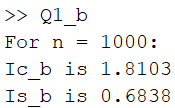
\includegraphics[width={0.4\linewidth}]{Q1_b_sol.png}
\end{multicols}
We can obverse that the error on [0,1] is \(\int_{0}^{1} w(x) - f(x) \,dx\) (Notice that \(w(x)\) is larger than \(f(x)\)). is will decrease by increasing n.
And the error on [h,1] will decrease by increasing n too.
For \(Ic\), the initial error is small because \(\lim_{x \to 0} \frac{f_{c}(x)}{w(x)} = 1\), So the error is small on [0,h]. But for \(Is\), the situation is the opposite.
\newline
For \(Ic\), Compare with data in (1-a) we can see \(Ic\) squeezed by \(Ic\) in (a) and (b). So when n is large enough, \(Ic_{a}, Ic_{b}\) will converge to the real Ic. (Here we don't considerate the rounding).
\newline
So it is a good way to approximate calculate Ic, but not work good for Is.
\rule[-0.7mm]{45em}{0.5pt}
%----------------(1-c)------------
\newline
(1-c)
\newline
Third, let's make a change of variables \(x = t^{2}\) and apply the composite trapezoidal rule. Now,
\[
  f_{c}(x) = g_{c}(t)={2\cos(t^{2})}\quad and \quad f_{s}(x) = g_{s}(t) = {2\sin(t^{2})}
\]
\[
  I_{c} = \int_{0}^{1} 2\cos(t^{2}) \,dt = \int_{0}^{1} f_{c}(x) \,dt \quad and \quad I_{s} = \int_{0}^{1} 2\sin(t^{2}) \,dt = \int_{0}^{1} g_{s}(t) \,dt
\]
\begin{multicols}{2}
\begin{verbatim}
function I = trapez_3a(f,n)
% assume f is vectorized
h = 1/n;
x = linspace(0,1,n+1);
I = f(x(1)) + f(x(end));
I = I + 2*sum(f(x(2:end-1)));
I = I*h/2;
end
\end{verbatim}
\columnbreak
\begin{verbatim}
n = 100:10:1000;
fc = @(t) 2.*cos(t.^2);
fs = @(t) 2.*sin(t.^2);
Ic_c = zeros(1,length(n));
Is_c = zeros(1,length(n));
index = 1;
for i = n
    Ic_c(index) = trapez_3a(fc,i);
    Is_c(index) = trapez_3a(fs,i);
    index = index+1;
end
save("1_c","Is_c","Ic_c");
\end{verbatim}
\end{multicols}

%第四页

\newpage
Then we plot \(I_{c}\) \(I_{s}\) depend on \(n\) (\(n\) can be hundards to 1000), And compare with the data from (1-a),(1-b)
\newline
\begin{verbatim}
n = 10:100;
Ic_c = zeros(1,length(n));
Is_c = zeros(1,length(n));
for i = n
    [Ic_c(i-9),Is_c(i-9)] = Q1_c(i.*10);
end
load("1_b.mat")
load("1_a.mat")
%plot
plot(n,Ic_c,'Color',"#D95319","LineWidth",1)
hold on
plot(n,Is_c,'Color',"#4DBEEE","LineWidth",1)
hold on
plot(n,Ic_b,'--','Color',"#A2142F","LineWidth",0.5);
hold on
plot(n,Is_b,'--','Color',"#0072BD","LineWidth",0.5)
hold on
plot(n,Ic_a,'--r',n,Is_a,'--b',"LineWidth",0.5);
axis([5 105 0.5 1.9]);
title('Change variables x = t^2');
xlabel('Intervals numbers');
ylabel('Integral result');
legend('Ic_c','Is_c','Ic_b','Is_b','Ic_a','Is_a','Location','East')
%save data for next question
save("1_c","Is_c","Ic_c");
\end{verbatim}
\begin{multicols}{2}
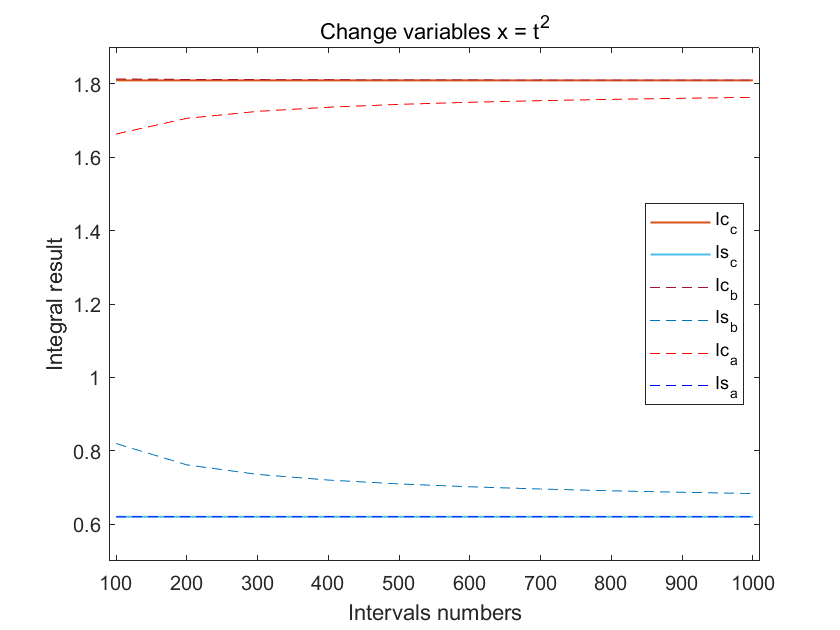
\includegraphics[width={\linewidth}]{Q1_c.png}
\columnbreak
\begin{verbatim}
fprintf('For n = 1000:\n...
Ic_c is %.4f\n...
Is_c is %.4f\n'...
,Ic_c(end),Is_c(end))
\end{verbatim}
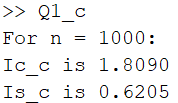
\includegraphics[width={0.4\linewidth}]{Q1_c_sol.png}
\end{multicols}

Because we don't have singularity now, so the integrals do not need to consider the error near the singularity.
It seems converge immediately. And is squeezed by the Integrals we calculate in (a) and (b).
\newline
It is a better way to remove the singularity for Is and Ic.
%第五页
\newpage
\rule[-0.7mm]{45em}{0.5pt}
%----------------(1-d)------------
\newline
(1-d)
\newline
Here I will use composite Simpson method, and then use Adapt Simpson method writing by loop.
\newline
Firstly, use the function in (C) and Composite Simpson
\begin{multicols}{2}
\begin{verbatim}
function I = simpson(f,n)
% n must be an even number
% f must be a vectorized
if mod(n,2)~=0
    warning...
    ("n must be a even number");
end
h = 1/n;
x = linspace(0,1,n+1);
I = f(0)+f(1)...
    +2*sum(f(x(3:2:n-1)))...
    +4*sum(f(x(2:2:n)));
I = I*h/3;
end
\end{verbatim}
\columnbreak
\begin{verbatim}
n = 100:10:1000;
fc = @(t) 2.*cos(t.^2);
fs = @(t) 2.*sin(t.^2);
Ic_d = zeros(1,length(n));
Is_d = zeros(1,length(n));
index = 1;
for i = n
    Ic_d(index) = simpson(fc,i);
    Is_d(index) = simpson(fs,i);
    index = index+1;
end
\end{verbatim}
\end{multicols}
Then plot and compare with (c) Similiarly:
\begin{verbatim}
load("1_c.mat");
subplot(2,2,1);plot(n,Ic_d);title("Composite Simpson of Ic");
subplot(2,2,2);plot(n,Ic_d,n,Ic_c);title("Compare Ic_c and Ic_d");
subplot(2,2,3);plot(n,Is_d);title("Composite Simpson of Is");
subplot(2,2,4);title("Compare Is_c and Is_d");plot(n,Is_d,n,Is_c);
\end{verbatim}
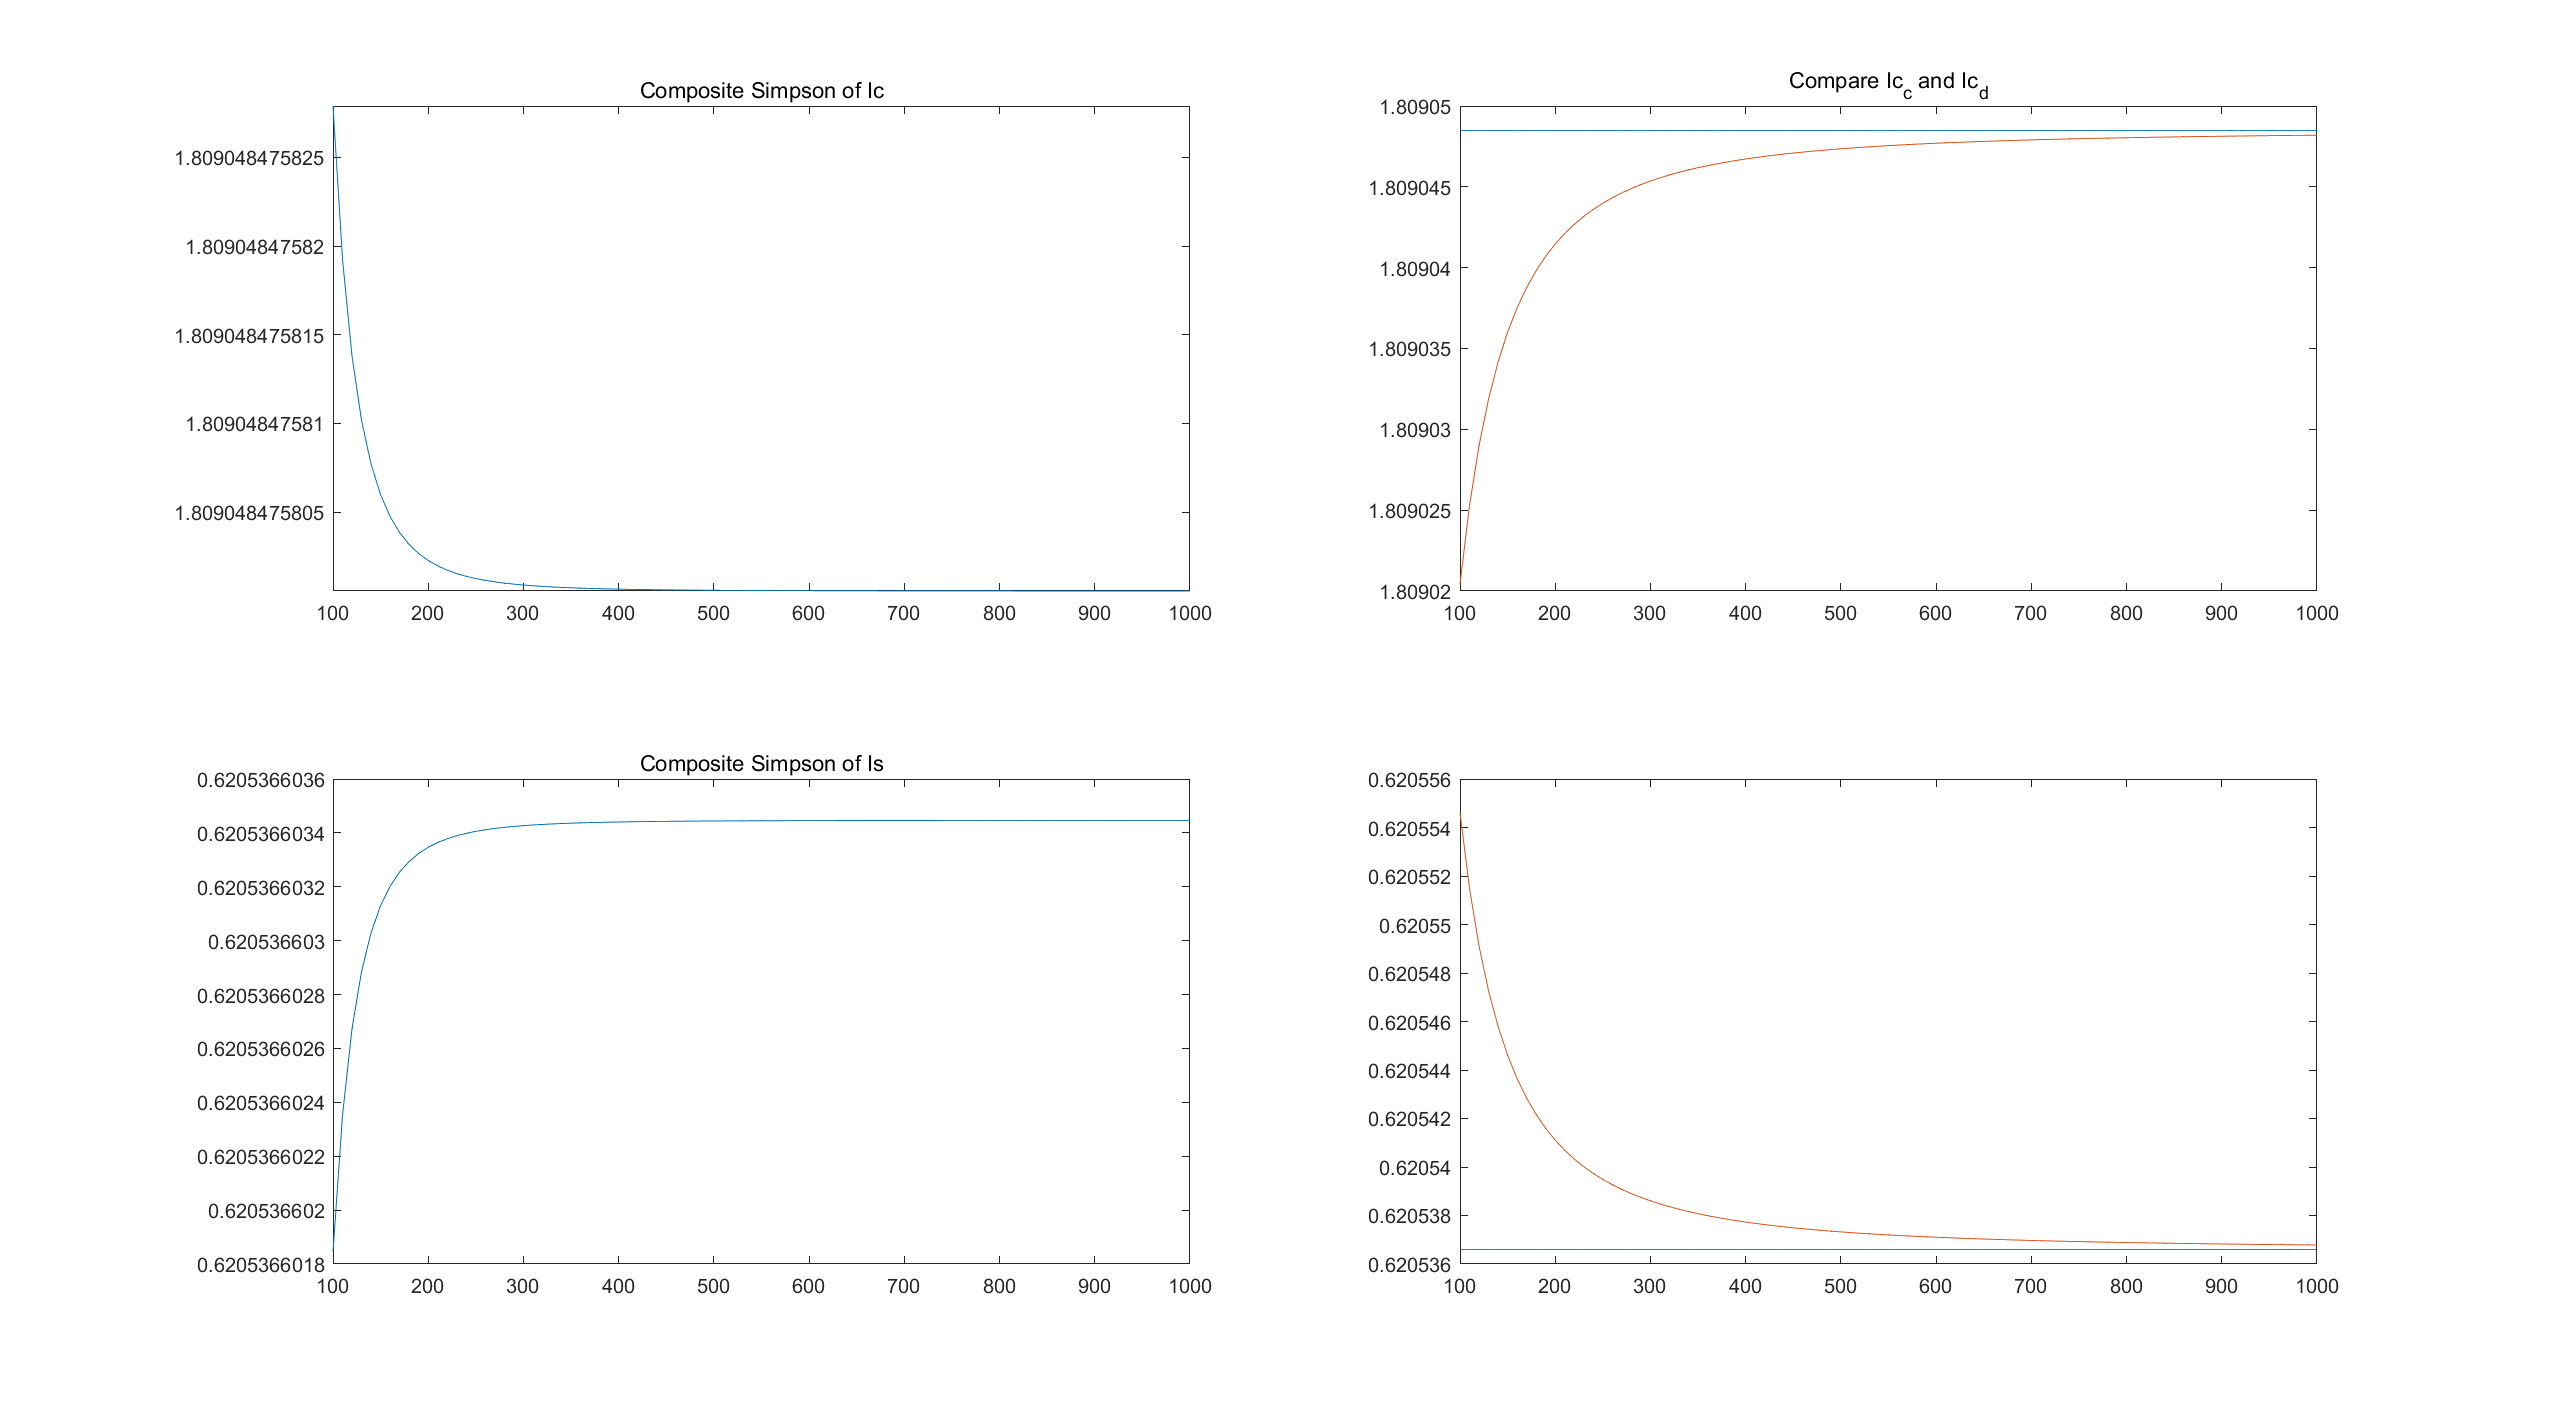
\includegraphics[width={\linewidth}]{Q1_d_CS.png}

\newpage
The picture has showed that the converge rate of Composite Simpson is much faster than the way we
\newline
used in (c).
\newline
Then we will show the Gauss-Legendre method to calculate it. The main function is similarity to simpson, you just need to change `\verb|simpson|' to `\verb|gauss|' in loop `for'.
And the total Gauss-Legendre function is too long, I will not post it here. But you can find it in the LAB codes.
Similar to the method we mentioned earlier, we can plot it:
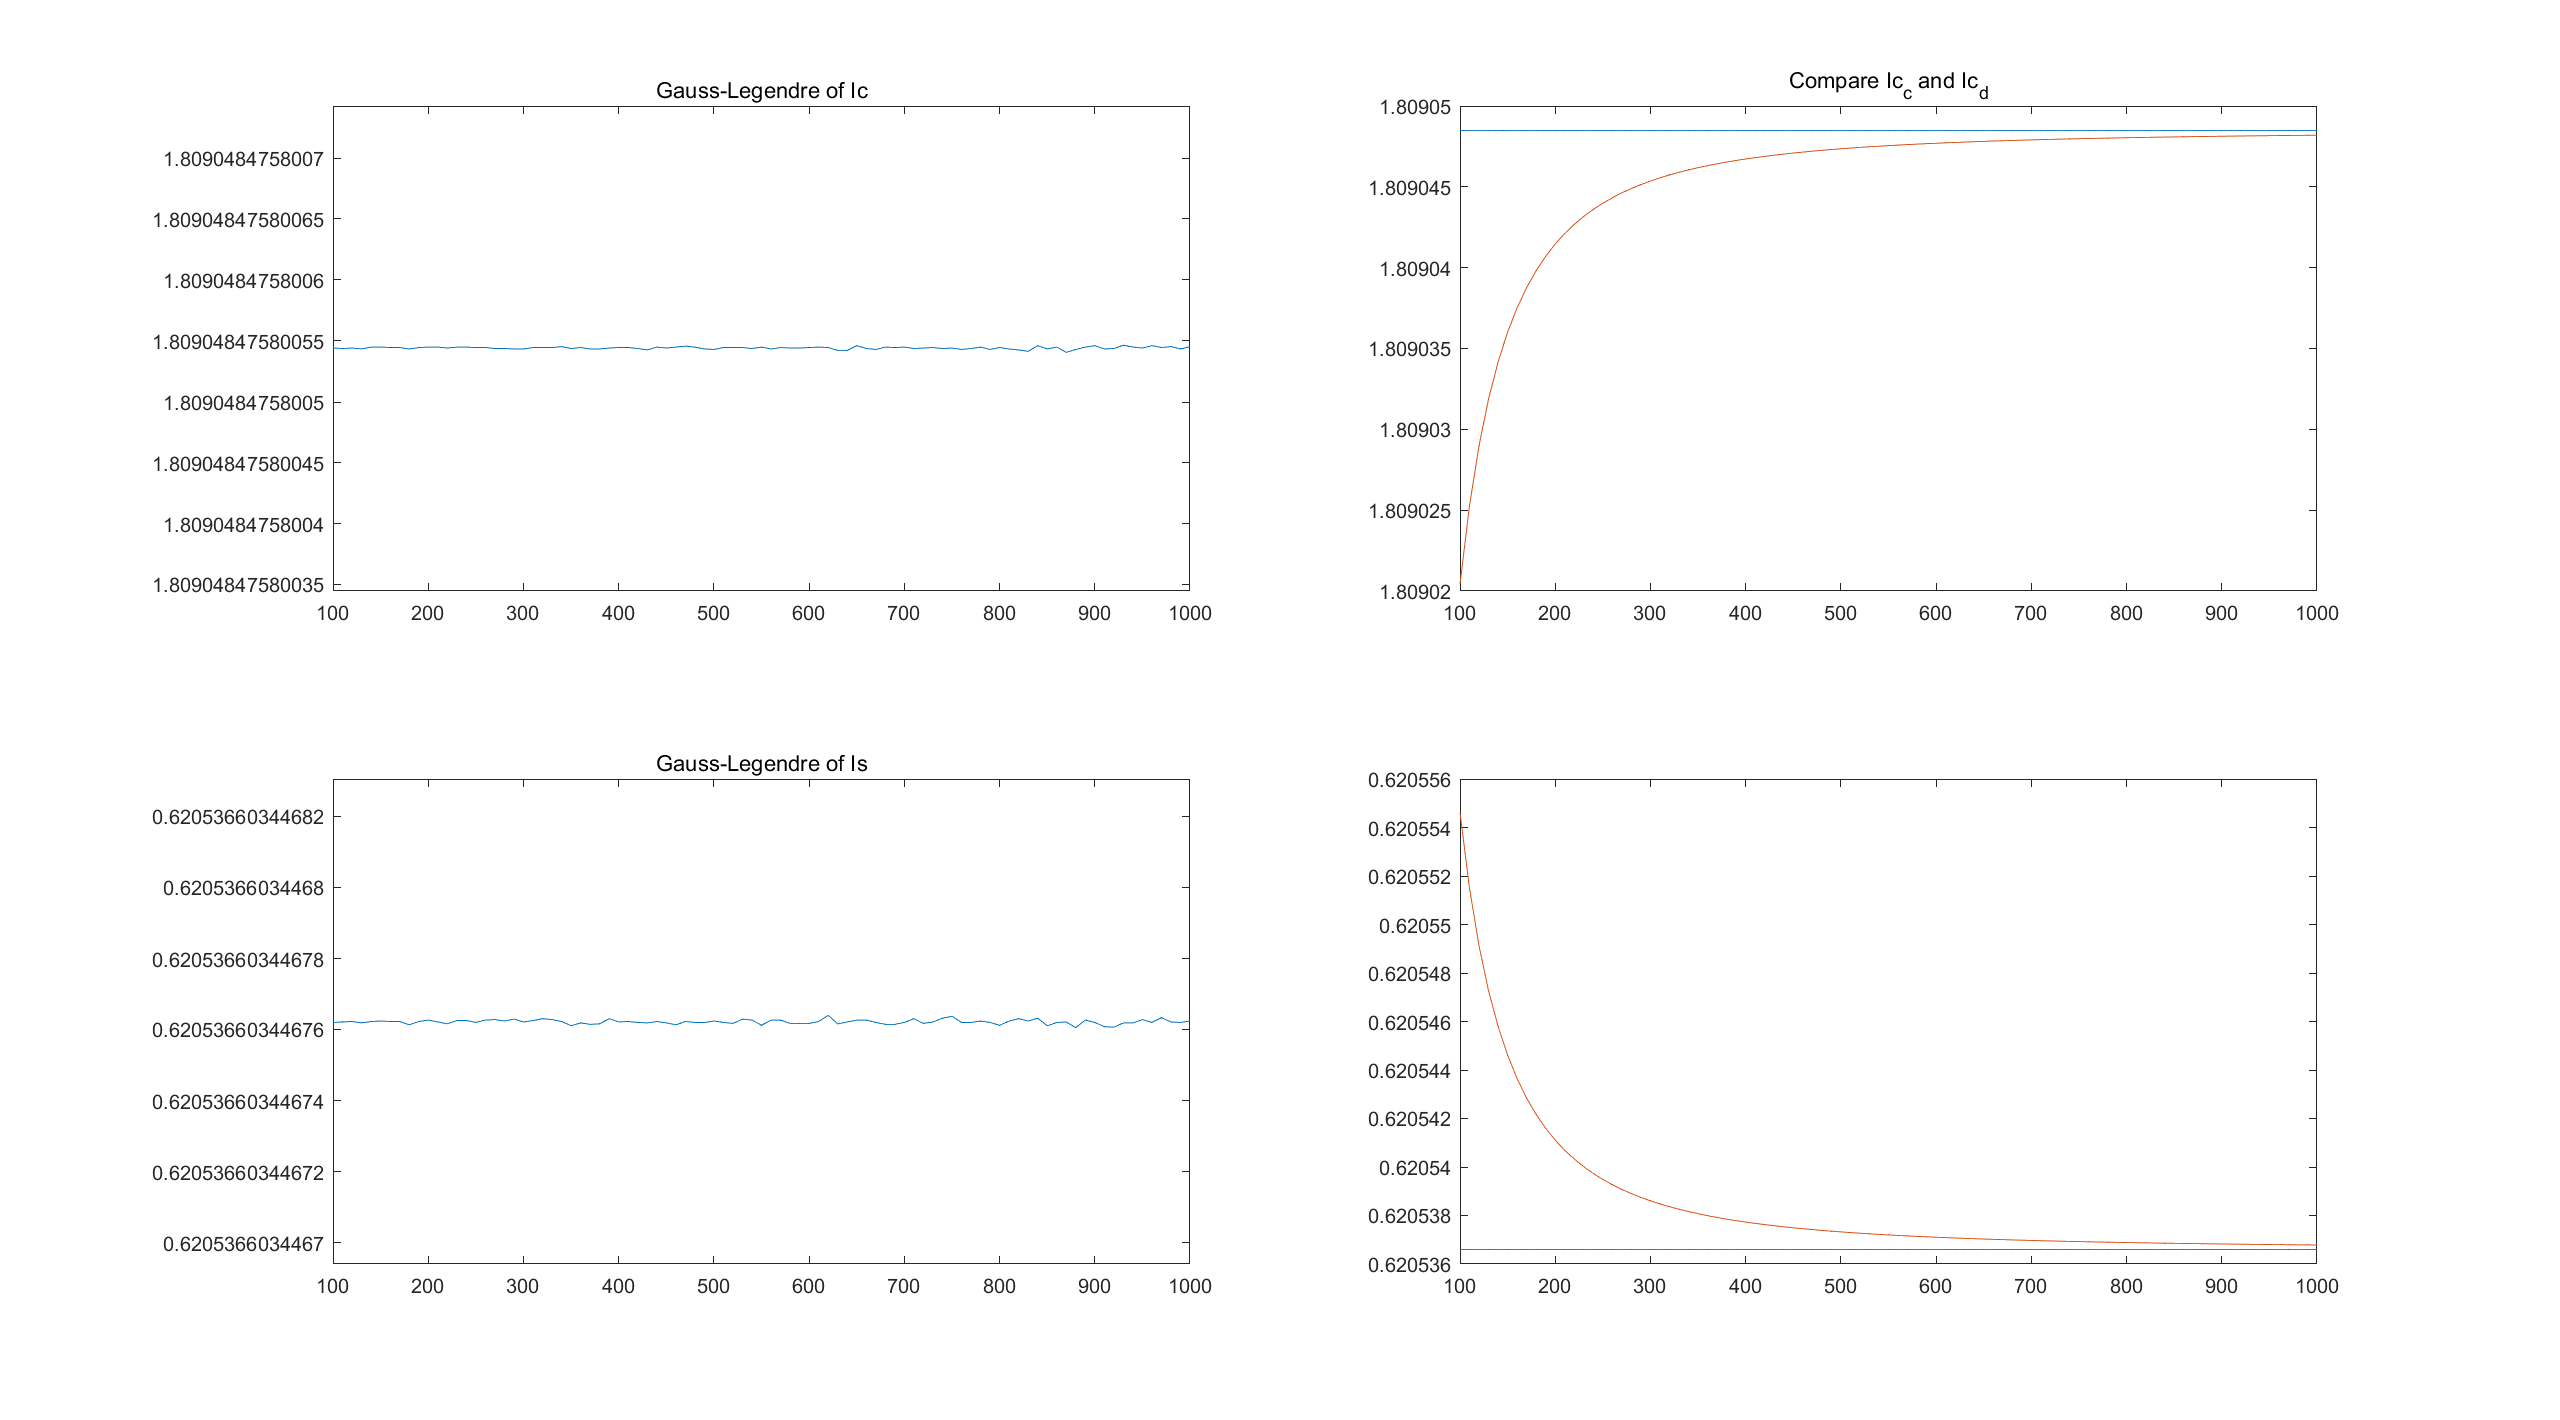
\includegraphics[width={\linewidth}]{Q1_d_GS.png}
It is obvisely that integral converge when n is just 100. So Gauss-Legendre seems better than Compose Simpson, especially n is not too big.
\newpage
\rule[-0.7mm]{45em}{0.1pt}
(Appendx of Q(1-d)) More explaination but maybe not useful to get marks.
\newline
But it still can't `control' the Approximate error we want. We don't know how big `n' is enough.
And if we just increasing n, computer may cost much more time to calculate it.
So we can chooose adapt method, like Sdapt Simpson method.
Here we just write it in loop way.

\begin{verbatim}
function [Q,err,sort_interval] = loopsimp(f,tinterval,tol)
subs = [tinterval(1:end-1);tinterval(2:end)];midpt = sum(subs)/2;
dif = diff(subs);subs_mid = [subs(1,:); midpt; subs(2,:)];
Ssub = 1/6.*dif.*([1,4,1]*f(subs_mid));Q = 0;interval = [];i=1;
while 1
    %calculate the error
    if isempty(subs)
        break;
    end
    midpt = sum(subs)/2;
    subs = reshape([subs(1,:); midpt; midpt; subs(2,:)],2,[]);
    dif = diff(subs);Sbig = Ssub;
    subs_mid = [subs(1,:); sum(subs)/2; subs(2,:)];
    Ssub = 1/6.*dif.*([1,4,1]*f(subs_mid));
    Ssub_accb = sum(reshape(Ssub,2,[]));err = abs(Sbig - Ssub_accb)/15;
    tol = tol/2;err_index = err < tol;
    suberr_index = reshape([err_index;err_index],1,[]);
    Q = Q + sum(Ssub_accb(err_index),'all');
    interval(:,i:i+sum(suberr_index)-1) = [subs(:,suberr_index)];
    i = i+sum(suberr_index);
    subs(:,suberr_index) = [];Ssub(:,suberr_index) = [];
end
[sort_interval(1,:),I] = sort(interval(1,:));
sort_interval(2,:) = interval(2,I);
end
\end{verbatim}
\begin{multicols}{2}
\begin{verbatim}
function [Ic,Is] = Q1_d_AS(tol)
% Adapt Simpson with loop
fc = @(t) 2.*cos(t.^2);
fs = @(t) 2.*sin(t.^2);
[Ic,~,~] = loopsimp(fc,[0,1],tol);
[Is,~,~] = loopsimp(fs,[0,1],tol);
end
\end{verbatim}
\columnbreak
\begin{verbatim}
i = 4:30;Q = 0.*i;err = 0.1.^i;
for j = i
    Q(j-3) = Q1_d_AS(err(j-3));
end
plot(Q);
xlabel("error less than n (1e-n)");
ylabel("Integral");
\end{verbatim}
\end{multicols}
For example, we want to calculate Ic, we can choose a not too big `Approximate Error', and directly get the integral:
\newline
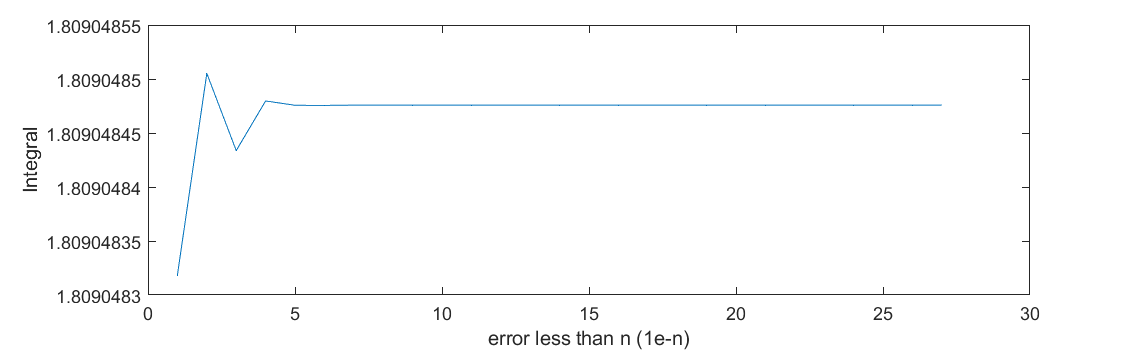
\includegraphics[width={0.7\linewidth}]{Q1_d_AS.png}
\newline
We can see it will converge immediately if we choose a not `too big' error.
\end{framed}
\newpage
%=================================第二题了
\item Question II: IVP.
\begin{framed}
We can substitute the value to get the differential equation, and ignore the units of these numbers
\[
  v^{'} = -9.8 - 0.002/0.11 \cdot v|v| = f(t,y), \quad v(0) = 80
\]
\rule[-0.7mm]{45em}{0.5pt}
%----------------(2-a)------------
(2-a)
\newline
Use Euler's method, and decrease the step sizes:
\begin{multicols}{2}
\begin{verbatim}
f = @(t,v) -9.8-0.002/0.11*v.*abs(v);
k = 1:100;n = 20.*2.^k;
err = inf(1,length(n));
FIRSTTIME = true;
for i = k
    [t, y] = eulerstep(f,0,20,n(i),80);
    if FIRSTTIME == true
        last_t=t;last_y=y;
        FIRSTTIME = false;
        continue
    else
        err(i-1) = max(abs( ...
            y(1:2:end)- last_y));
        if(err(i-1)<1e-4)
            t=last_t;y=last_y;
            err(i:end) = [];
            break
        end
        last_t=t;last_y=y;
    end
end
save("Q2_a",'t','y','err')
\end{verbatim}
\columnbreak
\begin{verbatim}
function [t, y] = eulerstep(f,a,b,n,ya)
% Euler explicit time-stepping
% y'=f(t,y), y(a) = ya
t = zeros(n+1,1); t(1) = a; 
h = (b-a)/n; d = numel(ya);
y = zeros(n+1,d); y(1,:) = ya;
for i = 1:n
    y(i+1,:) = y(i,:) + h*f(t(i),y(i,:));
    t(i+1) = t(i) + h;
end
\end{verbatim}
\end{multicols}
\begin{multicols}{2}
\begin{verbatim}
%% load data
load("Q2_a")
%% plot v(t)
plot(t,y,'b',"LineWidth",1);
xlabel("t(s)");ylabel("v(m/s)")
title("v(t)")
\end{verbatim}
\columnbreak
\begin{verbatim}
%% plot error
plot(err,'r',"LineWidth",1)
ax = gca;
ax.YScale = 'log';
xlabel("n");
ylabel("error")
title("error between h " + ...
    "and h/2 (h = 1/2^n)")
\end{verbatim}
\end{multicols}
\begin{multicols}{2}
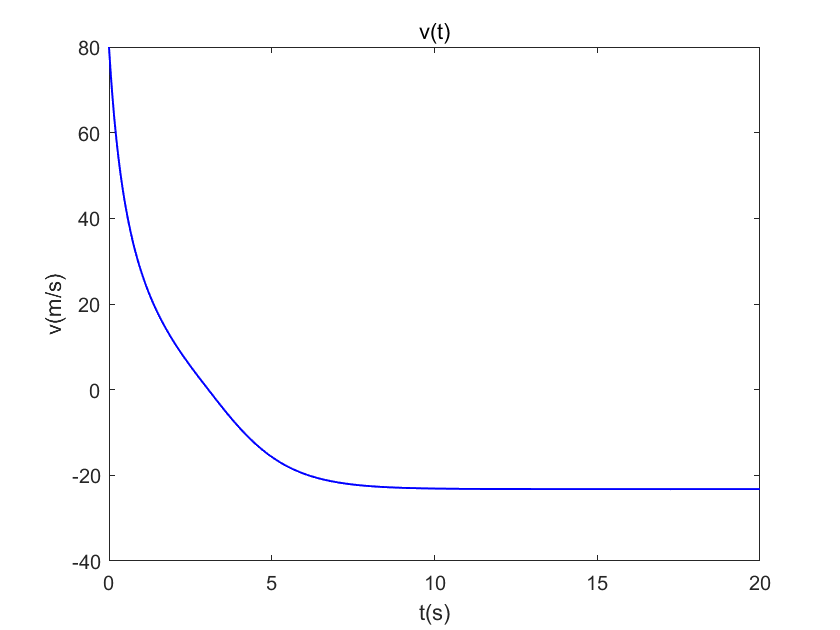
\includegraphics[width={\linewidth}]{Q2_a_2.png}
\columnbreak
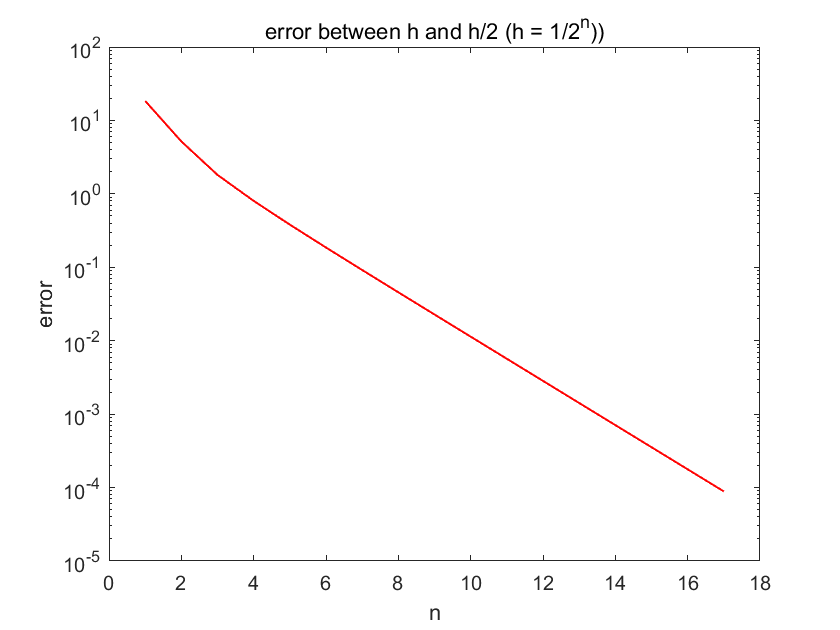
\includegraphics[width={\linewidth}]{Q2_a_e.png}
\end{multicols}



\newpage
\rule[-0.7mm]{45em}{0.5pt}
%----------------(2-b)------------
(2-b)
\newline
\textbf{Runge-Kutta method} is a family of iterative methods.
In general, an explicit s-stage Runge-Kutta method is of the form:
\begin{align*} 
  w_{0} &= \alpha\\
  k_{1} &= f(t{i},w_{i})\\
  k_{2} &= f(t{i}+hc_{2},w_{i}+ha_{21}k_{1})\\
  k_{3} &= f(t{i}+hc_{3},w_{i}+h(a_{31}k_{1}+a_{32}k_{2}))\\
  \vdots\\
  k_{s} &= f(t{i}+hc_{s},w_{i}+h(a_{s1}k_{1}+a_{s2}k_{2}+\cdots a_{s,s-1}k_{s-1}))\\
  w_{i+1}&=w_{i}+h(b_1k_1+b_2k_2+\cdots +b_sk_s)
\end{align*}
In this question, we will use 4-stage Runge-Kutta method, and control the error between h and h/2 just like Euler's mehod used in (2-a)
\begin{multicols}{2}
\begin{verbatim}
f = @(t,v) -9.8-0.002/0.11*v.*abs(v);
k = 1:100;n = 20.*2.^k;
err = inf(1,length(n));
FIRSTTIME = true;
for i = k
[t, y] = rkstep(f,0,20,n(i),80);
if FIRSTTIME == true
    last_t=t;last_y=y;
    FIRSTTIME = false;
    continue
else
    err(i-1) = max(abs( ...
        y(1:2:end)- last_y));
    if(err(i-1)<1e-4)
        t=last_t;y=last_y;
        err(i:end) = [];
        break
    end
    last_t=t;last_y=y;
end
end
save("Q2_b",'t','y','err')
\end{verbatim}
\columnbreak
\begin{verbatim}
function [t, y] = rkstep(f,a,b,n,ya)
% 4-stage Runge-Kutta 
% y'=f(t,y), y(a) = ya
t = zeros(n+1,1); t(1) = a; 
h = (b-a)/n; d = numel(ya);
y = zeros(n+1,d); y(1,:) = ya;
for i = 1:n
    k1 = h*f(t(i),y(i,:));
    k2 = h*f(t(i)+h/2,y(i,:)+k1/2);
    k3 = h*f(t(i)+h/2,y(i,:)+k2/2);
    k4 = h*f(t(i)+h,y(i,:)+k3);
    y(i+1,:)=y(i,:)+(k1+2*k2+2*k3+k4)/6;
    t(i+1) = t(i) + h;
end
\end{verbatim}
Then you can plot it similarity in Q(2-a) plot codes. Just change \verb|load "Q2_a"| to \verb|load("Q2_b")"|.
\end{multicols}
\begin{multicols}{2}
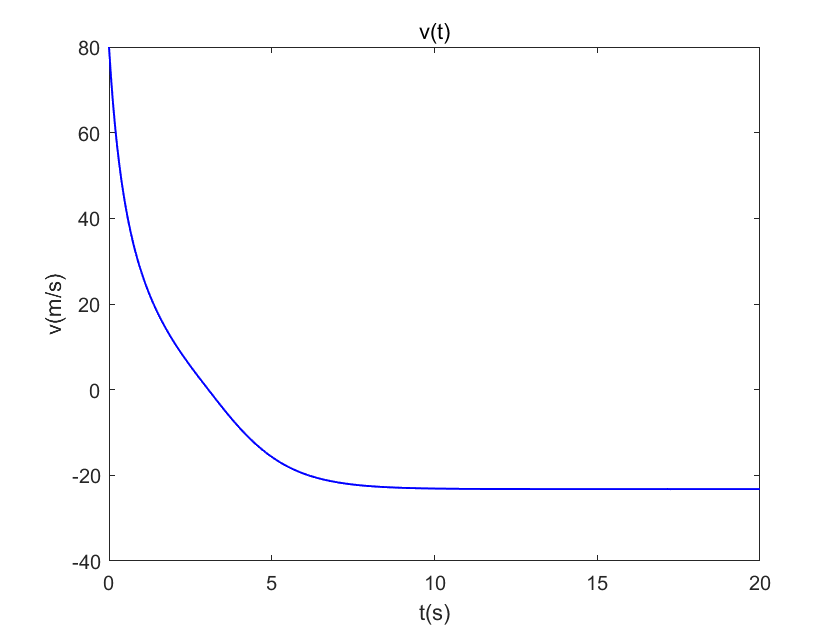
\includegraphics[width={\linewidth}]{Q2_b.png}
\columnbreak
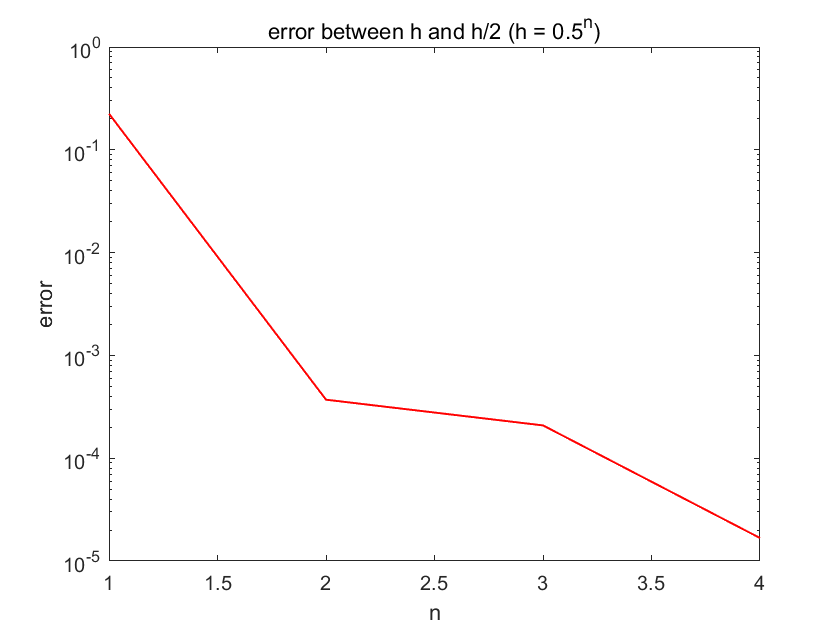
\includegraphics[width={\linewidth}]{Q2_b_e.png}
\end{multicols}

\newpage%第九页

In the same error control, Comparing from the output:
\newline
In Euler's method, we can see that final \(h = 7.629394531250000e-06\), which is \(2^{-17}\), it means it iterated many times, and the length of t and y calculated will be very big, is 5242881. The data will use more memory to store.
\newline
but in 4-stage Runge Kutta, the final \(h= 0.0625\), which is \(2^{-4}\), is means it iterated shorter times, and the length of t and y calcuulated will be smaller, is 641. The data will use less memory to store.
\newline
Comparing from the running time:
\newline
In Euler's method, running time for error <1e-4 in my computer is 0.637615s.
\newline
In in 4-stage Runge Kutta, running time for error <1e-4 in the same computer is 0.00989s. Is much shorter.
\newline
(notice test it for 100 times and take average)
\rule[-0.7mm]{45em}{0.5pt}
%----------------(2-c)------------
(2-c)
\newline
It is obviously that the ``easy way'' is connect the distrete `y' to be a function. For example use \verb|construct = griddedInterpolant(t,y);| and \verb|f = @(t) construct(t);| (Notice that I first construct the construct to avoid creating it too each time when you want to use the function).
And then use the function in LAB code `bisect' and `trapeze'. But I think it is boring and not the clever idea. Because you need to use the `not basic' function provided by matlab. So I rewrite the \verb|bisect.m| and \verb|trapeze.m| to make it work for discrete data.
\newline
The projectile reachs its maximum height when its `v' is zero. So we can use bisection to find the smallest interval [a,b], and y(a)>0, y(b)<0. Then use the linear interpolation to find the approximate `t', \(v(t) = 0\)
\begin{multicols}{2}
\begin{verbatim}
load("Q2_a.mat")
[a,b] = bisect(y);
tt = -y(a).*(t(b)-t(a))./...
    (y(b)-y(a))+t(a);
\end{verbatim}
\columnbreak
\textbf{Here we can get tt = 3.05212 which is the approximate time the projectile reachs its maximum height.}(Function bisection is showed below).
\end{multicols}
Then we need to integrals it to find the maximum height. Here we will use composite trapez method. Firstly, we will calculate it peace by peace, and then add them step by step:
\begin{multicols}{2}
\begin{verbatim}
function [a,b] = bisect(y)
% find root boundary
% ab is the index through 0
a = 1;b = length(y);
if y(a)*y(b) > 0 
    error(['f(a) and ' ...
        'f(b) must have ' ...
        'different signs']);
end
while b-a > 1
    if y(a)==0||y(b)==0
        break
    end
    mid = floor((a+b)/2);
    if y(a)*y(mid) > 0
        a = mid;
    else
        b = mid;
    end
end
end
\end{verbatim}
\columnbreak
\begin{verbatim}
function I = trapeze_eacht(y,t)
y = y(:)';
h = t(2)-t(1);
subinterval = [y(1:end-1);y(2:end)];
I = [1,1]*subinterval*h/2;
end
\end{verbatim}

\begin{verbatim}
function int_I = sigema(I)
int_I = 0.*I;
Q = 0;
for i = 1:length(I)
  Q = Q+I(i);
  int_I(i) = Q;
end
end
\end{verbatim}
\end{multicols}

\newpage


\begin{multicols}{2}
\begin{verbatim}
load("Q2_a.mat")
[a,b] = bisect(y);
tt = -y(a).*(t(b)-t(a))./...
    (y(b)-y(a))+t(a);
I = trapeze_eacht(y,t);
int_I = sigema(I)+500;
plot(t,int_I,'r','LineWidth',1)
title("The height changed by t")
xlabel("t(s)")
ylabel("H(t)(m)")
axis([0 8 400 600]);
max_height=max(int_I(a),int_I(b));
\end{verbatim}
\textbf{Here we can get maximum height, which is 570.276869(m) for tt = 3.05212(s)}
\columnbreak
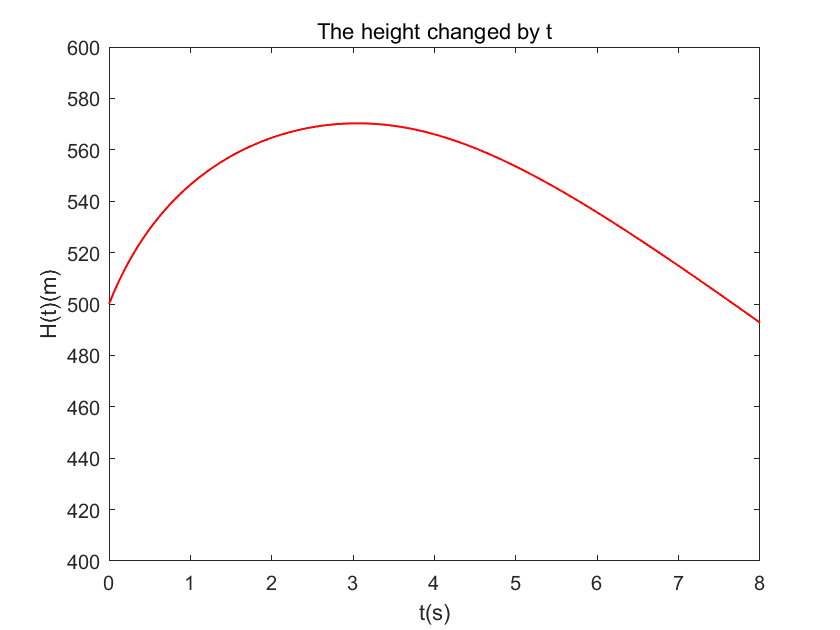
\includegraphics[width={\linewidth}]{Q2_c_h.png}
\end{multicols}
Then we can know the projectile reaches the maximum height 570.276869(m) at the time 3.05212(s).
\newline
Then lets make sure the errors are less than \(10^{-4}\):
\newline
Let's assume the our approximate for v is very approximate, it means not consider the error created by Euler's method.
In the bisect method, because we use the data calculated in (2-a), the h here is \(2^{-17}\). So our error boundary is \((0+20)/2^{17}=1.5259e-04\) which is less than \(10^{-4}\).
So computed time is less than \(10^{-4}\).
In the error term for the composite Trapezoidal rule:
\[
v^{''} = -0.002 \cdot 2v\cdot v^{'}=-0.004v\cdot (-9.8-0.002v^{2})< 10, \quad 80> v> 0
\]
\[
\frac{b-a}{12}h^{2}v^{''}(\mu) < \frac{20}{12} \cdot 2^{-34} \cdot 10 = 9.7e-10 \ll 1e-4
\]
\newline
So the height are less than \(10^{-4}\).

\newpage

\rule[-0.7mm]{45em}{0.5pt}
%----------------(2-d)------------
(2-d)
\newline
Now we need to extend the simulation time from [0,20] to [0,40].
The code is similarity to the (Q2-b) just change the \verb|[t, y] = rkstep(f,0,20,n,80);| to \verb|[t, y] = rkstep(f,0,40,n,80);|. and then we can use the functions we written in (Q2-c):
\begin{multicols}{2}
\begin{verbatim}
load("Q2_b.mat")
I = trapeze_eacht(y,t);
int_I = sigema(I);
[a,b] = bisect(int_I+500);
t_between=t([a,b]);
t_middle =sum(t_between)./2;
plot(t,int_I,'r','LineWidth',1)
title("The height changed by t")
xlabel("t(s)")
ylabel("H(t)(m)")
\end{verbatim}
\columnbreak
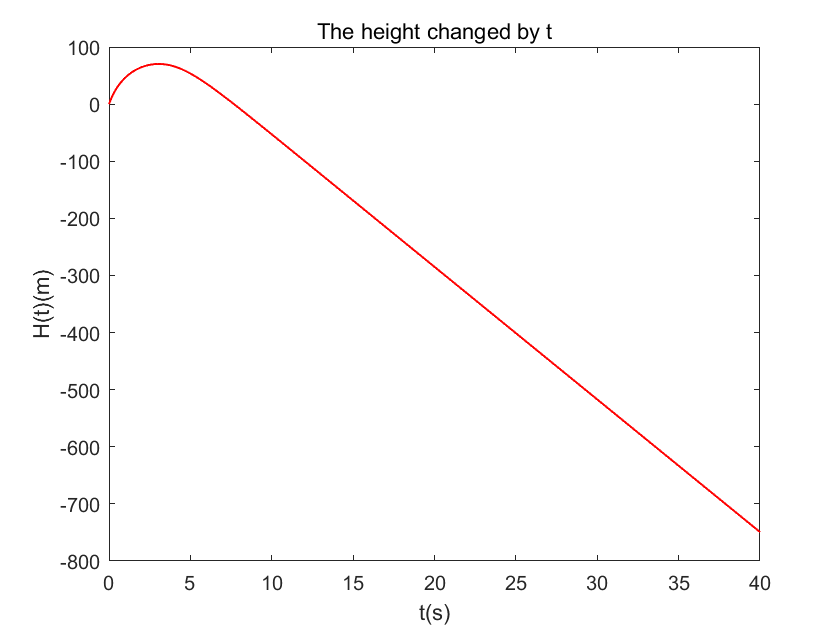
\includegraphics[width={0.9\linewidth}]{Q2_d_h.png}
\end{multicols}
\textbf{Here we can get the time it hits the earth is between 29.25 and 29.28125. We can choose the middle time as approximate, which is 29.265625(s).}
\end{framed}
\end{enumerate}
\end{flushleft}

\hfill\today
\hrule
\hrule

%***************************************************************************
\vfill
\end{document}